% All the theory behind the program
\section{Background theory}

\subsection{Introduction}

This section presents theoretical background, numerical examples, and explanation for implementing the program library \prog. This suite of algorithms, developed at the UBC-Geophysical Inversion Facility, is needed to invert DC potentials and IP responses over a 2-D earth structure. The manual is designed so that a geophysicist who has an understanding of DC resistivity and Induced Polarization field experiments, but who is not necessarily versed in the details of inverse theory, can use the codes and invert his or her data.

A typical DC/IP experiment involves inputting a current \textit{\textbf{I}} to the ground and measuring the potential away from the source. In a time-domain system the current has a duty cycle which alternates the direction of the current and has off-times between the current pulses at which the IP voltages are measured. A typical time-domain signature is shown in Figure \ref{fig:basicTime}. In this Figure, $\phi_\sigma$ is the potential that is measured in the absence of chargeability effects. This is the ``instantaneous'' value of the potential measured when the current is turned on. In mathematical terms this potential is related to the electrical conductivity, $\sigma$, by:
%
\begin{equation}
\label{eq:genFwd}
\phi_\sigma = \mathcal{F}_{dc}[\sigma],
\end{equation}
%
where the forward mapping operator $\mathcal{F}_{dc}$ is defined by the equation
%
\begin{equation}
\nabla \cdot (\sigma\nabla\phi_\sigma) = - \mathbf{I}\delta(r-r_s),
\label{eq:dcForward}
\end{equation}
%
and also by appropriate boundary conditions. In equation \ref{eq:dcForward}, $\sigma$ is the electrical conductivity in Siemens/meter (S/m), $\nabla$ is the gradient operator, $\mathbf{I}$ is the strength of the input current in Amperes, and $r_s$ is the location of the current source. For typical earth structures, $\sigma$, while positive, can vary over many orders of magnitude. The potential $\phi_\sigma$ in equation \ref{eq:dcForward} is the potential due to a single current. This is the value that would be measured in a pole-pole experiment. If potentials from pole-dipole or dipole-dipole surveys are to be generated then they can be obtained by using equation \ref{eq:dcForward} and the principle of superposition. 

When the earth material is chargeable the measured voltage will change with time and reach a limit value which is denoted by $\phi_\eta$ in Figure \ref{fig:basicTime}. There are a multitude of microscopic polarization phenomena, which collaborate so that this final value is achieved but all of these effects can be consolidated into a single macroscopic parameter called ``chargeability''. We denote chargeability by the symbol $\eta$. Chargeability is dimensionless, positive, and confined to the region [0,1). 
%
\begin{figure}
\centering
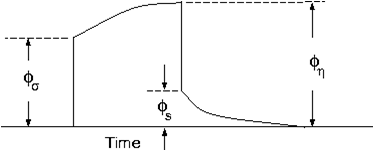
\includegraphics[width=0.5\columnwidth]{eta}
\caption{Definition of the three potentials associated with DC/IP experiments.}
\label{fig:basicTime}
\end{figure}
%

To carry out forward modelling to compute $\phi_\eta$ we adopt the formulation of \citet{Siegel59}, which says that the effect of a chargeable ground is modelled by using the dc resistivity forward mapping, $\mathcal{F}_{dc}$, but with the conductivity replaced by $\sigma = \sigma(1-\eta)$. Thus:
%
\begin{equation}
\label{eq:phiEta}
\phi_\eta = \mathcal{F}_{dc}[\sigma(1-\eta)],
\end{equation}
%
or 
%
\begin{equation}
\label{eq:ipForward}
\nabla \cdot (\sigma(1-\eta)\nabla\phi_\sigma) = - \mathbf{I}\delta(r-r_s).
\end{equation}
%
The IP datum, which we refer to as ``apparent chargeability'' is defined by
%
\begin{equation}
\eta_a = \frac{\phi_s}{\phi_\eta} = \frac{\phi_\eta - \phi_\sigma}{\phi_\eta},
\label{eq:genApCharge}
\end{equation}
%
or
%
\begin{equation}
\eta_a = \frac{\mathcal{F}_{dc}[\sigma(1-\eta)] - \mathcal{F}_{dc}[\sigma]}{\mathcal{F}_{dc}[\sigma(1-\eta)]}.
\label{eq:genApChargeDC}
\end{equation}
%
Equation \ref{eq:genApChargeDC} shows that the apparent chargeability can be computed by carrying out two DC resistivity forward modelling routines with conductivities $\sigma$ and $\sigma(1-\eta)$. Note that in this definition apparent chargeability is dimensionless and, in the case of data acquired over an earth having constant chargeability $\eta_o$, we have $\eta_a = \eta_o$.

The field data from a DC/IP survey are a set of $N$ potentials (ideally $\phi_\sigma$, but usually $\phi_\eta$) and a set of $N$ secondary potentials $\phi_s$ or a quantity that is related to $\phi_s$. The goal of the user is to utilize these data to acquire quantitative information about the distribution of the two physical parameters of interest: conductivity $\sigma(x,y,z)$ and chargeability $\eta(x,y,z)$.

The distribution of conductivity and chargeability in the earth can be extremely complicated. Assuredly earth structure is 3D, but for the DC/IP codes developed here we restrict ourselves to 2D structures and assume that the survey has been carried out along a traverse that is perpendicular to strike. The cross-section of the earth is divided into rectangular prisms each having a constant value of conductivity and chargeability. 

\subsection{Forward modelling}
The forward modelling for the DC potentials and IP apparent chargeabilities and secondary potentials is accomplished using a finite difference technique to solve equation \ref{eq:dcForward}. The program which performs this calculation is \codeName{DCIPF2D}. In Version \version~we include the option to calculate IP data by multiplying the sensitivity matrix $\mathbf{J}$ by the chargeability provided by user. That is, we forward model with the linear equations that will be used for the inversion. The chargeability in this case can have arbitrary units. The forward modelled data are calculated as
%
\begin{equation}
\bvec{d}_{ip} = \bvec{J}_{ip}\eta,
\end{equation}
where $\bvec{d}_{ip}$ is the IP data and $\bvec{J}_{ip}$ is the sensitivity matrix for the IP problem:
\begin{equation}
\bvec{J}_{ip} = -\frac{\partial \ln\phi_\eta}{\partial \ln\sigma} = -\frac{1}{\sigma_\eta}\frac{\partial\phi_\eta}{\partial \ln\sigma} = -\frac{1}{\bvec{d}_{dc}}\bvec{J}_{dc},
\label{eq:sensIP}
\end{equation}
given DC data, $\bvec{d}_{dc}$. Forward modeling using equation \ref{eq:sensIP} is further explained in the section \ref{invIPdataSection}.

\subsection{General inversion methodology}
The computing programs outlined in this manual solve two inverse problems. In the first we invert the DC potentials $\phi_\sigma$ to recover the electrical conductivity $\sigma(x,z)$. This is a non-linear inverse problem that requires linearization of the data equations and subsequent iteration steps. Next, we invert IP data to recover the chargeability $\eta(x,z)$. Because chargeabilities are usually small quantities $(\eta < 0.3)$ it is possible to linearize equation \ref{eq:genApChargeDC} and derive a linear system of equations to be solved. Irrespective of which data set is being inverted however, we basically use the same methodology to carry out the inversions.

To outline our methodology it is convenient to introduce a single notation for the \fileName{data} and for the \fileName{model}. We let $\bvec{d} = (d_1,d_2,\ldots,d_n)^T$ denote the data so that $d_i$ is the i$^{th}$ potential in a DC resistivity data set or the i$^{th}$ apparent chargeability in an IP survey. Let the physical property of interest be denoted by the symbol $m$. The quantity $m_j$ can denote the conductivity or chargeability for the j$^{th}$ cell. For the inversion we choose $m_j = \ln(\sigma_j)$, when inverting for conductivities and $m_j = \eta_j$ when reconstructing the chargeability section.

The goal of the inversion is to recover a model vector $\bvec{m} = (m_1,m_2,\ldots,m_m)^T$, which acceptably reproduces the $n$ observations $\bvec{d}^{obs} = (d_1^{obs},d_2^{obs},...,d_n^{obs})^T$. Importantly, the data are noise contaminated, therefore we don't want to fit them precisely. A perfect fit in our case would be indicative, that incorrect earth model is recovered, as some features observed in the constructed model would assuredly be artifacts of the noise.

Alternatively, if we fit the data too poorly then information about the conductivity that is coded in the data will not have been recovered. Our objective therefore is to neither under-fit nor over-fit the data. Rather, we want to find a model that reproduces the data only to within an amount that is justified by the estimated uncertainty in the data. To accomplish this we introduce a global misfit criterion:
%
\begin{equation}
\label{eq:phid}
\psi_d = \left\| \mathbf{W}_d(\mathbf{G}\mathbf{m}-\mathbf{d})\right\|^2.
\end{equation}
%
where $\bvec{W}_d$ is a data weighting matrix. In this work, we shall assume that the noise contaminating the i$^{th}$ observation is an uncorrelated Gaussian random variable having zero mean and standard deviation $\epsilon_i$. As such, an appropriate form for the $N \times N$ matrix is $\bvec{W}_d = diag\left\{1/\epsilon_1,\ldots,1/\epsilon_n\right\}$. With this choice, $\psi_d$ is the random variable distributed as chi-squared with $N$ degrees of freedom. Its expected value is approximately equal to $N$ and accordingly, $\psi_d^*$, the target misfit for the inversion, should be approximately equal to this value. 

It is common to use an $l_2$ norm measure of data fit as shown in equation \ref{eq:phid}. However, the Huber norm \cite[]{Huber64} has been incorporated to handle outliers in the data. The general form of the Huber norm is
\begin{equation}
\label{eq:Huber}
\tau(y) = \begin{cases}
y^2 & |y| \leq c \\
2c|y| - c^2 & |y| > c.
\end{cases}
\end{equation}
From equation \ref{eq:Huber}, let $y=\textbf{W}_d(\textbf{G}\mathbf{m}-\textbf{d})$ and the data misfit function then becomes
\begin{equation}
\label{eq:Huber_phid}
\Phi_d = \sum_{i=1}^n \begin{cases}
\left[ {\textbf{W}_d}^i(\textbf{G}_i\mathbf{m}-{d_i}) \right] ^2 & |y_i| \leq c \\
2c|{\textbf{W}_d}^i(\textbf{G}_i\mathbf{m}-{d_i})|-c^2 & |y_i| > c.
\end{cases}
\end{equation}
where $c$ is a constant that separates the elements of vector $y$ into those considered large and those that are considered small \cite[]{FarquharsonOldenburg98}. 

Earth conductivity distributions are complex. To allow maximum flexibility to produce a model of arbitrary shape it is important that $M$, the number of cells representing the model, is large. In our inversions, $M$ will almost always be greater than $N$, the number of data. The inverse problem therefore reduces to finding a set of $M$ model parameters using only $N$ data constraints under the condition that $M > N$. Clearly the solution is no unique and this non-uniqueness represents the principle obstacle for obtaining unambiguous information about earth structure from the observations.
 
Any inversion algorithm (if it works) will produce a model, which reproduces the data. But there are infinitely many possible models. So which one does the algorithm produce? It is not good practice to let the program make a random selection. Rather, a responsible approach is to direct the inversion algorithm to produce a model that is geologically reasonable and is constrained by additional information if such information is available. This can be implemented by formulating a ``model objective function'' which, when minimized, produces a model with desirable characteristics. The critical aspect of the inversion is therefore to form the model objective function which we characterize by $\psi_m$. To do this, the user must ask the question ``what type of model is desired?'' Should the model be smooth or should it be blocky? Is there a reference or background model that the constructed model should emulate? If there is a reference model, is it better known in some places than others so that the constructed model should be close to the reference model in certain locations but can depart from our preconceived ideas in other areas? Whatever the answer to these questions, a guiding philosophy should always be to find a model which (in some sense) is ``as simple as possible.'' The non-uniqueness inherent in the inversion generally means that we can generate models which are arbitrarily complicated. We cannot however, make models that are arbitrarily simple. For example, a half space will generally not reproduce data acquired from a geophysical survey. 

In the inversion algorithms in \programName, our choice for the objective function $\psi_m$ is guided by a desire to find a model which has minimum structure in the vertical and horizontal directions and at the same time is close to a reference model $m_o$. To accomplish this, we minimize a discretized approximation to 
%
\begin{eqnarray}
\psi_m(m,m_o) = &\alpha_s \int\int w_s(x,z)(m-m_o)^2 dxdz + \nonumber \\
&\int \int \left\{ \alpha_x w_x(x,z) \left( \frac{\partial(m-m_o)}{\partial x} \right)^2 + \alpha_z w_z(x,z)\left( \frac{\partial(m-m_o)}{\partial z} \right)^2 \right\} dxdz
\label{eq:intMOF}
\end{eqnarray}
%
In equation \ref{eq:intMOF}, the functions $w_s,w_x,w_z$ are specified by the user and the constant $\alpha_s$ controls the importance of closeness of the constructed model to the reference model $m_o$ and $\alpha_x,\alpha_z$ controls the smoothness of the model in the two directions. Varying the ratio $\alpha_x/\alpha_z$ allows the construction of models that are smoother, thus more elongated, in either $x-$ or $z-$direction. The discrete form of \ref{eq:intMOF} is the following:
%
\begin{eqnarray}
\psi_m &&= (\bvec{m}-\bvec{m}_o)^T\left\{ \alpha_s \mathbf{W}_s^T\mathbf{W}_s+\alpha_x \mathbf{W}_x^T\mathbf{W}_x+\alpha_z \mathbf{W}_z^T\mathbf{W}_z \right\} (\bvec{m}-\bvec{m}_o), \nonumber \\
&&\equiv (\bvec{m}-\bvec{m}_o)^T\mathbf{W}_m^T\mathbf{W}_m(\bvec{m}-\bvec{m}_o)^T, \\
\label{eq:shortMOF}
&&= \norm{\mathbf{W}_m(\bvec{m}-\bvec{m}_o)}^2.
\label{eq:disMOF}
\end{eqnarray}
%
If $w_s, w_x,$ and $w_z$ are set equal to unity, then $\bvec{W}_s$ is a diagonal matrix with elements $\sqrt{\Delta x \Delta z}$, where $\Delta x$ is the length of the cell and $\Delta z$ is its thickness, $\bvec{W}_x$ has elements $\sqrt{\Delta z / dx}$ where $dx$ is the distance between the centres of horizontally adjacent cells, and $\bvec{W}_z$ has elements $\sqrt{\Delta x / dz}$ where $dz$ is the distance between the centres of vertically adjacent cells.

For blockier models, we have incorporated the measure proposed by Ekblom (\citeyear{Ekblom73,Ekblom87}) that has been found to be useful. The generalized version is given as
\begin{equation}
\label{eq:Ekblom}
\tau(y) = (y^2 + \epsilon^2)^{\frac{\rho}{2}},
\end{equation}
where $\epsilon$ is some positive number. The smaller $\epsilon$ becomes, the measure tends towards the $l_\rho$ norm. Large values of $\epsilon$ tend the measure to behave like a scaled sum-of-squares. For the model objective function in equation \ref{eq:shortMOF}, $y = \bvec{W}_m(\bvec{m} - \bvec{m}_o)$ and the system of equations is solved with the projected gradients through a chi-factor regularization. The resulting model objective function is 
%
\begin{eqnarray}
\psi_m &&= \left[(\bvec{m} - \bvec{m}_o)^T\alpha_s\bvec{W}^T_s\bvec{W}_s(\bvec{m} - \bvec{m}_o) + \epsilon^2\right]^{\frac{\rho}{2}} + \left[(\bvec{m} - \bvec{m}_o)^T\alpha_x\bvec{W}^T_x\bvec{W}_x(\bvec{m} - \bvec{m}_o) + \epsilon^2 \right]^{\frac{\rho}{2}} \nonumber \\
&&+ \left[(\bvec{m} - \bvec{m}_o)^T\alpha_z\bvec{W}^T_z\bvec{W}_z(\bvec{m} - \bvec{m}_o) + \epsilon^2 \right]^{\frac{\rho}{2}}.
\label{eq:ekblom}
\end{eqnarray}
%
Details of the Eklom norm within the context of geophysical inversion can be found in \cite{FarquharsonOldenburg98}. 

It should be noted that in equation \ref{eq:disMOF}, the reference model can be removed from the spatial ($x$ and $z$) components. The effect is that the reference model places emphasis on the magnitude of the model, but its spatial variations do not influence the spatial derivatives. The model objective function becomes
\begin{equation}
\psi_m = (\bvec{m}-\bvec{m}_o)^T\left(\alpha_s \mathbf{W}_s^T\mathbf{W}_s\right)(\bvec{m}-\bvec{m}_o) + \bvec{m}^T\left\{\alpha_x \mathbf{W}_x^T\mathbf{W}_x+\alpha_z \mathbf{W}_z^T\mathbf{W}_z \right\}\bvec{m}
\label{eq:mofNOref}
\end{equation}
%
and for the Ekblom norm
%
\begin{eqnarray}
\psi_m &&= \left[(\bvec{m} - \bvec{m}_o)^T(\alpha_s\bvec{W}^T_s\bvec{W}_s)(\bvec{m} - \bvec{m}_o) + \epsilon^2 \right]^{\frac{\rho}{2}} \nonumber \\
&&+ \left[\bvec{m}^T(\alpha_x\bvec{W}^T_x\bvec{W}_x)\bvec{m} + \epsilon^2 \right]^{\frac{\rho}{2}} + \left[\bvec{m}^T(\alpha_z\bvec{W}^T_z\bvec{W}_z)\bvec{m} + \epsilon^2 \right]^{\frac{\rho}{2}}.
\end{eqnarray}
This is a new feature in \codeName{DCIP2D} and gives the user greater flexibility. 
% 

The inverse problem is now properly formulated as an optimization problem: 
%
\begin{align}
\label{eq:inverseProblem}
& \mbox{minimize } \psi_m(\bvec{m},\bvec{m}_o)&=\norm{\mathbf{W}_m(\bvec{m}-\bvec{m}_o)}^2 \\ \nonumber
& \mbox{subject to } \psi_d(\bvec{d},\bvec{d}^{obs})&=\norm{\mathbf{W}_d(\bvec{d}-\bvec{d}^{obs})}^2 =\psi_d^*.
\end{align}

In equation \ref{eq:inverseProblem}, $\bvec{m}_o$ is a starting model and $\bvec{W}_m$ is a general weighting matrix which is designed so that a model with specific characteristics is produced. The minimization of $\psi_m$ yields a model that is close to $\bvec{m}_o$ with the metric defined by $\bvec{W}_m$ and so the characteristics of the recovered model are directly controlled by these two quantities. If the data errors are Gaussian and their standard deviations have been adequately estimated then the target misfit should be $\psi_d^* = N$. The data misfit function can take the form of the $l_2$ norm as shown above or the Huber norm from equation \ref{eq:Huber_phid}.

\subsection{Inversion of DC data}
The inversion of the apparent resistivity data is carried out using the program \codeName{DCINV2D}. The inversion of DC resistivity data formulated as the minimization in equation \ref{eq:inverseProblem} is nonlinear since the data do not depend linearly upon the conductivity model. We tackle this problem using a Gauss-Newton approach in which the objective function is linearized about a current model, $m(n)$, and a model perturbation is solved for and used to update the current model. Substituting $m(n+1) = m(n)+m$ into the objective function in equation \ref{eq:inverseProblem}
%
\begin{equation}
\psi(\bvec{m} + \delta \bvec{m}) =  \left\| \mathbf{W}_d\left( \mathcal{F}_{dc}[\bvec{m}^{(n)}] + \bvec{J}\delta\bvec{m} - \mathbf{d}\right)\right\|^2 + \beta \left\| \bvec{W}_m\left(\bvec{m} + \delta\bvec{m} - \bvec{m}_o\right) \right\|^2 + H.O.T.,
\end{equation}
where $\bvec{J}$ is the sensitivity matrix and the element $J_{ij}$ quantifies the influence of the model change in jth cell on the ith datum such that
%
\begin{equation}
\bvec{J} = \frac{\partial d_i}{\partial m_j} = \frac{\partial \phi_i}{\ln \sigma_j}.
\end{equation}

Neglecting the higher order terms and setting to zero the derivative with respect to $\delta m$ yields
%
\begin{equation}
\label{eq:GN}
\left( \bvec{J}^T\bvec{J} + \beta \bvec{W}_m^T\bvec{W}_m \right) \delta \bvec{m} = -\bvec{J}^T \left( \mathcal{F}_{dc}[\bvec{m}^{(n)}] - \bvec{d} \right) - \beta\bvec{W}_m^T\bvec{W}_m \left(\bvec{m}^{n} - \bvec{m}_o \right).
\end{equation}
Here we assume that the matrix $\bvec{W}_d$ has been absorbed into the sensitivity matrix and data vectors. This is the basic equation that is solved to obtain the model perturbation. The new model is then generated by
%
\begin{equation}
\bvec{m}^{(n+1)} = \bvec{m}^{(n)} + \gamma\delta\bvec{m},
\end{equation}
where $\gamma \in (0,1]$ limits the step size and is chosen to ensure that the total objective function is reduced.


\subsection{Inversion of IP data}
\label{invIPdataSection}
To invert IP data, we first linearize equation \ref{eq:genApCharge}. Let $\eta_j$ and $\sigma_j$ denote the respective chargeability and electrical conductivity of the j$^{th}$ cell. Linearizing the potential $\phi_\eta$ about the conductivity model $\sigma$ yields: 
%
\begin{equation}
\phi_\eta = \phi(\sigma - \eta\sigma)=\phi(\sigma) - \sum\limits_{j=1}^M\frac{\partial\phi}{\partial\sigma_j}\eta_j\sigma_j + H.O.T.
\end{equation}
%
The above equation is then substituted into equation \ref{eq:genApCharge}:
%
\begin{equation}
d = \frac{\phi_\eta-\phi_\sigma}{\phi_\eta} = \frac{-\sum\limits_{j=1}^M\frac{\partial\phi}{\partial\sigma_j}\eta_j\sigma_j}{\phi(\sigma)- \sum\limits_{j=1}^M\frac{\partial\phi}{\partial\sigma_j}\eta_j\sigma_j}.
\end{equation}
%
This can be approximately written as
%
\begin{equation}
d = -\sum\limits_{j=1}^M\frac{\sigma_j}{\phi}\frac{\partial\phi}{\partial\sigma_j}\eta_j = -\sum\limits_{j=1}^M\frac{\partial \ln\phi}{\partial\ln\sigma_j}\eta_j,
\end{equation}
%
and therefore the i$^{th}$ datum is
%
\begin{equation}
d_i = \sum\limits_{j=1}^M\bvec{J}_{ij}\eta_j,
\label{eq:ithIPdat}
\end{equation}
%
where
\begin{equation}
\bvec{J}_{ij} = -\frac{\partial\ln\phi_i[\sigma]}{\partial\ln\sigma_j}
\label{eq:IPJij}
\end{equation}
%
is the sensitivity matrix. Our inversion problem is formulated as 
%
\begin{eqnarray}
\mbox{minimize } &\psi_m = \norm{\bvec{W}_m(\eta-\eta_o)}^2 \nonumber \\
\mbox{subject to } &\psi_d=\norm{\bvec{W}_d(\bvec{J}\eta-\bvec{d}^{obs})}^2,
\label{eq:IPphi}
\end{eqnarray}
%
where $\psi_d^*$ is a target misfit. In reality the true conductivity $\sigma$ is unknown and so we use the conductivity recovered from the inversion of the DC resistivity data to construct the sensitivity matrix elements in equation \ref{eq:IPJij}. 

The functional in equation \ref{eq:IPphi} can be minimized directly but we need to ensure that the recovered chargeability is positive. In the inversion of the DC potentials to recover the conductivity we ensured positivity by working with $\ln(\sigma)$ as the model in the inversion and applying the model norm to this quantity. This is justified, since conductivity varies over many orders of magnitude and it is the variation of conductivity that is diagnostic of earth structure. Intrinsic chargeability is confined to the region $[0,1)$. Moreover, we are not generally interested in the variation of chargeability in the range between zero and some small number (e.g., 0.01). Working with logarithmic values however, puts undue emphasis on these small values. An efficient method by which to solve the linear inverse problem with positivity constraints is through a non-linear mapping of variables. More details of the IP inversion algorithm can be found in \cite{OldenburgLi94}. 
